%!TEX program = xelatex
% 使用 ctexart 文类,UTF-8 编码
\documentclass{article}
  \usepackage{xeCJK,indentfirst}
  \usepackage{amsfonts, amsmath, amssymb}
  \usepackage{graphicx}
  \usepackage[normalem]{ulem}

    \newtheorem{theorem}{Theorem}[section]
  \newtheorem{lemma}{Lemma}  
  \newtheorem{definition}{Definition}[section]
  \newtheorem{proof}{Proof}[section]  
  \numberwithin{equation}{section}

    \newcommand{\bra}[1]{\langle #1 |}
  \newcommand{\ket}[1]{| #1 \rangle}
  \newcommand{\bracket}[2]{\langle #1 | #2 \rangle}
  \newcommand{\bracketl}[3]{\langle #1 | #2 | #3 \rangle}
  \newcommand{\func}{\mathrm \,}
  \newcommand{\define}[2]{
   \begin{definition}
    \begin{description}
    \item[#1]
    #2
   \end{description}
   \end{definition}
  }
  \newcommand{\mean}[1]{\langle #1 \rangle}

  \newcommand{\sch}{Schr\"odinger} 
  \newcommand{\grad}{\nabla}

  \setlength{\parindent}{2em}
  \setlength{\textheight}{240mm}
  \setlength{\textwidth}{155mm}
  \setlength{\oddsidemargin}{0mm}
  \setlength{\evensidemargin}{0mm}
  \setlength{\topmargin}{-20mm}
  \renewcommand{\baselinestretch}{1.2}
  \title{王林军老师课题组本科生入门指南}
  \author{Chaoqun ZHANG-张超群\\Rui LI - 李睿}
  \date{\today}
  \begin{document}
    \maketitle
    \tableofcontents
    \newpage
    \section{引言}
  \begin{quote}
    老师说``这个东西很简单''的时候,往往是普通化学本科生搞不定的东西。
    \begin{flushright}
      ————李睿,在抱怨化学本科生编程能力不够时的调侃
    \end{flushright}
  \end{quote}
  \begin{quote}
    你有问题就要问,你如果不问,我就默认你都会了。
    \begin{flushright}
      ————王林军老师
    \end{flushright}
  \end{quote}

  欢迎进入王林军老师的课题组!无论您是由于何种原因,出于什么目的,来到王林军老师的课题组足以证明了您的勇气!\sout{看,在王林军老师组的都很休闲的}

  由于王林军老师研究比较``底层''的计算化学,所以会对数学、物理、计算机等知识内容会有更高的要求。而历届在王老师做事的本科生们都不止一次地抱怨来王老师的课题组的门槛非常高,而且没有合适的入门指南,使得难度进一步提高(\sout{你会发现你听了一年组会都学不到什么东西}),同时化学系对数理方面的要求实在不敢恭维,从而刚参加王老师的组会的时候会近乎100\%地出现``这是什么/我是谁/我在干什么''的疑惑,因此编者们共同商量,觉得出一份入门指南非常的重要,于是草草编写了这样的一份。

  另外,本组有与之配套的入门训练,但是暂时由于种种原因没有对每个本科生展开,所以在阅读本指南时,也可以花时间接触本组关于代码书写(行星运动)和势间跳跃方法(Tully文章)的
  基本训练,关于后者我们在指南中略有涉及,但是具体的代码实现还要靠自己的练习才行。由于并非专业科研文章,此指南在参考文献方面会比较欠缺,但是偶尔举出的几篇文章仍然
  推荐读者阅读相关内容,对理解本指南和王老师课题组的工作都有一定帮助。本指南将主要为王老师组的非绝热动力学方向服务,王老师课题组还有其他的研究方向,
  比如全局优化问题,机器学习相关和固体材料性质的计算等,这些内容在本指南中不作专门的讨论。
  
  简而言之,本指南旨在为诸位不同时间加入王林军老师课题组或者感兴趣的同学们提供一个深入了解的机会,因此很多内容不追求深度,编者认为,对于决定在这里完成毕设或者
  深造的同学来说,本指南只是一个入门皮毛。另外,编者们水平有限,如果有错误也是正常现象,望读者海涵。

    \section{Linux基础及服务器使用}
    Linux和macOS、Windows并称为三大电脑操作系统,都是用来完成用户和计算机之间的互动。Linux由于其出色的稳定性以及免费(相对于Unix系统),被广泛用于服务器的操作系统。当然Linux是存在图形界面的,但它的最为使用,也最为核心的部分还是它的终端,也就是字符界面。为了如何操作这玩意儿,一些基础知识是必须的。

    \subsection{连接至服务器}
    王林军老师课题组是使用浙大西溪校区的超级计算机集群来进行日常的工作的,简单地就叫服务器。听起来非常高大上,我们所编写的程序(或者商业软件)在普通计算机上当然也可以运行,只是很多时候
    需要过分长的时间,还要保持电脑全天开机,基本是不可能的,因此我们需要交给集群处理。

    集群计算机的操作系统都是Linux系统,我们需要用自己的个人电脑连接到服务器上,这样可以实现对服务器的远程操作,如果你的个人电脑是Linux或者mac系统,可以直接
    在终端使用ssh命令登录服务器,但是由于组内工作电脑和多数个人电脑为Windows系统,这一部分我们暂时不作展开,有兴趣的同学可以直接网上搜索。在Windows系统下连接
    Linux服务器,需要通过一些软件的辅助,比如PuTTY和XSHELL,鉴于后者有不少优势,比如更加新人友好\sout{并且好看},我们就以后者举例。

    XSHELL目前有官方的中文网站\footnote{https://www.netsarang.com/zh/xshell/},可以找到学生用的免费版,下载XSHELL和XFTP两个软件,
    前者是一个在Windows操作系统下实现ssh功能的软件,用于连接远程服务器;后者是实现sftp功能的软件,用于服务器和本地计算机之间的文件传递。
    这两个软件可以满足在理论计算化学组连接远程服务器的一切需求。安装好之后打开XSHELL,如下图所示新建会话,
    \begin{center}
      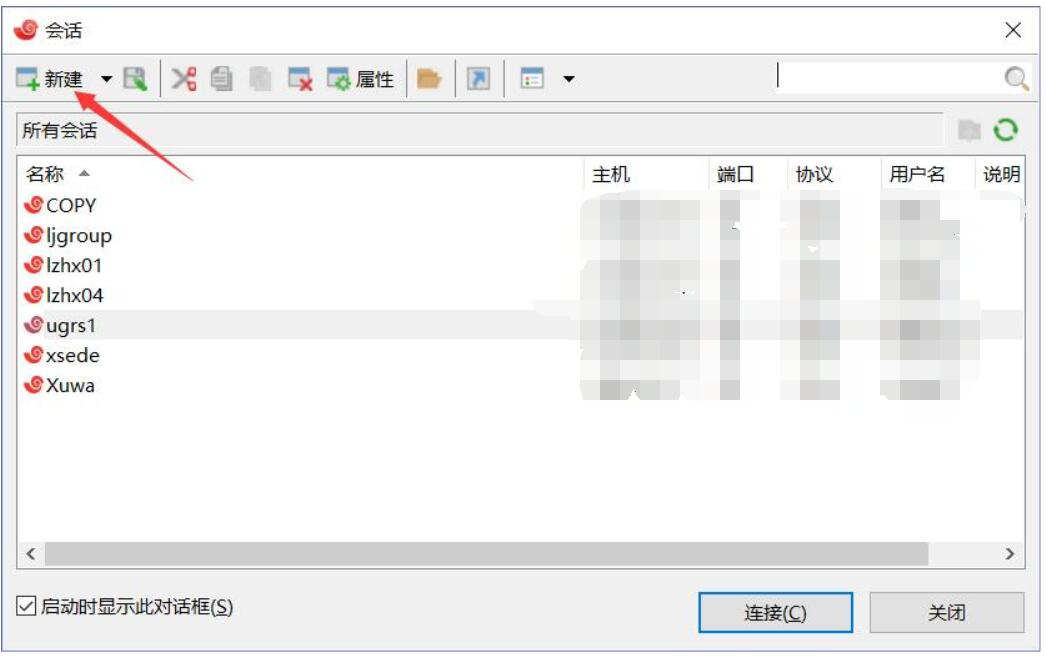
\includegraphics[width = 10cm]{fig/xshell1.jpg}
      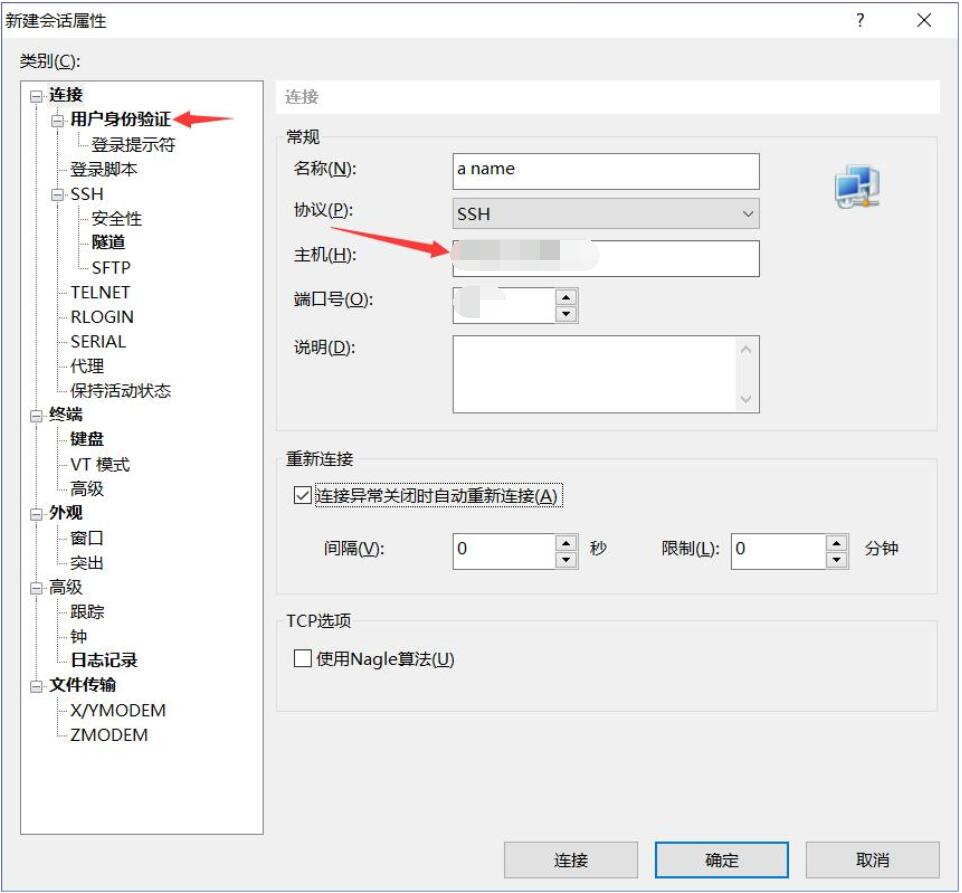
\includegraphics[width = 8cm]{fig/xshell2.jpg}
    \end{center}
    随便起个名字,主机填入10.22.51.200(注意:想要成功连接该IP需要浙大内网:ZJUWLAN、有线网络或者RVPN均可),端口号默认22,在用户身份验证界面
    用户名输入ugrs3\_LJ,密码为linjungroup\footnote{这个是专为入门本科生注册的账号,主要供学习使用,毕设或者读研读博正式在组内工作会有新的账号}。
    此时如果见到类似下图的界面,就代表已经成功登陆进我们的服务器,并处于\textbf{主目录}下。
    \begin{center}
      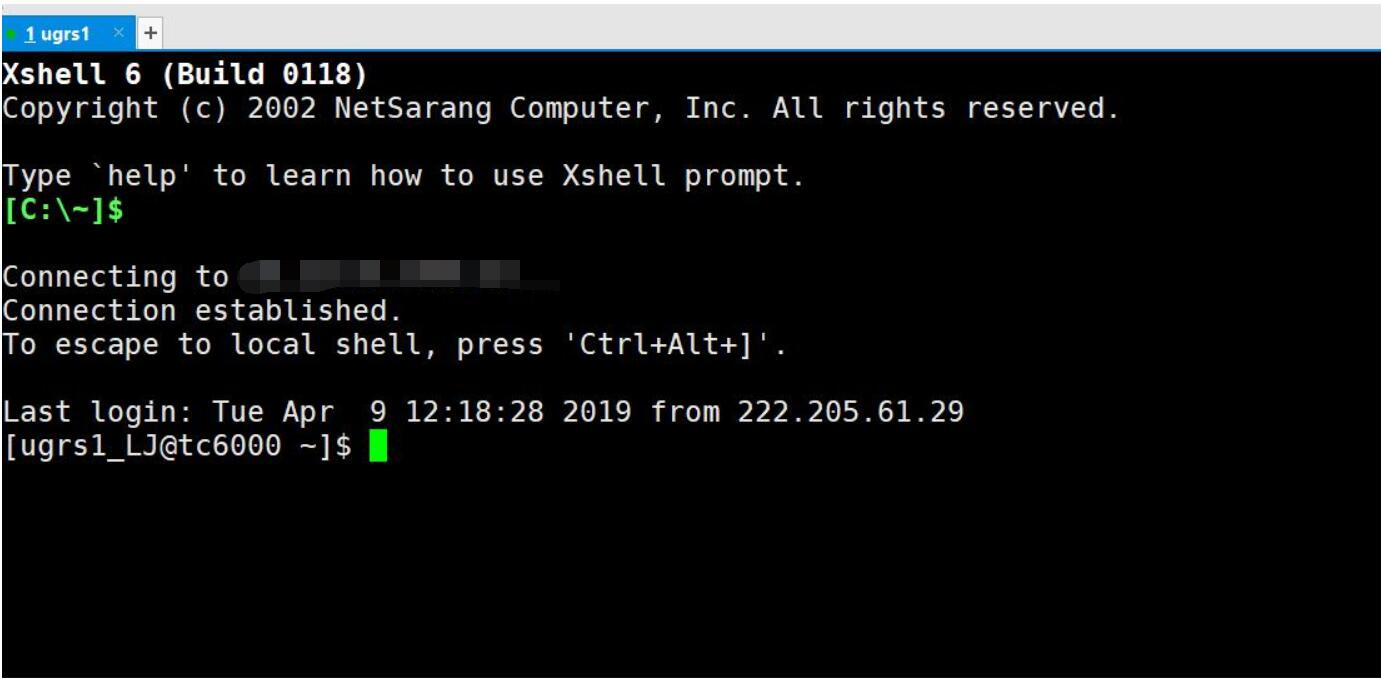
\includegraphics[width = 10cm]{fig/xshell3.jpg}
    \end{center}
    登录服务器之后,就可以按照下一小节的内容进行操作,学习Linux系统的各类指令,和如何在Linux系统下编辑文件,
    为了安全起见,我们建议每个读者在主目录建立自己的文件夹,然后再自己的文件夹中进行各种操作,避免对他人的文件误操作而造成损失。

    \subsection{Linux基本操作}
    \begin{description}
    \item[cd]
      进入输入目录的文件夹;
      `cd folder/'
      P.S : `cd ..' 返回上一级文件夹
    \item[ls]
      列出所在文件夹的子文件夹;

    \item[vi / vim]
      打开文件查看内容;vim事实上是一个文本编辑器(比方说这个文档的一部分也是用vim编辑的)

      P.S :输入不存在的文件可直接创立该文件;

    vim有一个梗,就是几乎所有的人刚上手的时候都不知道{\textbf 该怎么退出}。在这里面稍微描述一下最基本的使用方法:
    \begin{description}
      \item[i / Ins] 如果已经打开了某个文本,那么这两个键中的一个能够允许你对文本作出修改。它左下角会显示 ``--INSERT--'' 这样的文段,这说明你处在编辑模式,这时候你按出的大部分操作会如同你使用大部分文本编辑器的时候一样,会完整地呈现在你正在修改的文本上。
      \item[Esc] 无论你处在何种模式,按了Esc你就能回到正常模式,在该模式下你可以用它自身的快捷键来直接作出一些修改,也可输入命令来完成别的操作(比如{\textbf 退出})。

      \item[:q!] 这里`:'表示进行对vim程序自身的命令,`q'是quit,`!'表示强制。也就是输了这个命令并按回车后会强制退出并不保存文件。

      \item[:wq] 以此类推,这个表示的是保存并退出。没错,`:w'就是进行保存,并不退出。
    \end{description}
    好了,现在你也是会用vim的人了!跟我一起喊,\sout{vim天下第一!}
    \item[pwd]
      显示所在目录路径;它会显示所处目录的绝对路径,而这个绝对路径是你在任何别的目录下都能访问的。从该角度出发,事实上别的几乎所有操作都可以指定绝对路径(比如简单的访问,或者复制,或者在程序里面调用/生成文件)。

    \item[mkdir]
      在所在目录下建立文件夹:
      `mkdir levest' 表示建立名字为`levest'的文件夹

    \item[cp] 复制文件至某个目录
      `cp einfield.com slot' 表示将`einfield.com' 在`slot'文件夹下进行粘贴

    \item[mv] 原则上它表示将某个东西移动到什么地方,但它的另一个神奇操作在于它可以重命名文件/文件夹(后缀还是要加好)。

    \item[rm] \textbf{ 危险!}这是表示删除操作。

    \item[-r] 在Linux中大部分的`-*' 表示了所进行的主要命令的附加指令(附加属性,\sout{buff})。像这里`-r'一般用来表示是对整个文件夹进行操作,像上面的cp, rm 都可以加上-r。

    \item[*] *一般在Linux表示缺省符号,也就是在这里面可以填任何东西。比方说,`rm *.c' 表示任何后缀为`.c'的文件都会被删除\footnote{这就是为什么sudo rm -rf /* 这个梗会流行的原因。}。

    \end{description}

    读者可以在登录之后所在的主目录下先输入ls和回车,看到当前目录下的文件和文件夹,然后输入“mkdir 文件夹名”的方式创建属于自己的文件夹,然后cd自己的文件夹,之后再这个目录
    下进行后续的操作。
    \subsection{使用服务器递交任务}
    我们的超算集群,简单地说是由很多的CPU(\textbf{节点})构成的,每个CPU有28个\textbf{核},据说服务器的单核运行效率其实是低于正常个人计算机的,但是优势在计算资源非常多。
    西溪校区的超算集群主要是王林军老师和洪鑫老师出资,也主要是这两个课题组在使用。王老师占有其中的48个节点,共1344个核。
    这些节点按照一定的顺序组合成了两个\textbf{队列},分别为ljcluster和ljtest,前者又可以分为wenchang和quantum,使用ljclustat指令可以看到
    全组的节点使用情况。尽管是为本科生学习练习使用的账号,ugrs3\_LJ账号仍然有对服务器三个节点的访问权限(即ljtest队列)。
    我们在服务器上递交任务,就是将自己的程序交给这些核去运算,要实现这个靠的是PBS任务管理系统。
    
    TODO

    \section{数学基础}
    \subsection{线性代数回顾及变分法}
    数学基础的第一小节将关注于最基础的数学内容,主要是线性代数的一些知识,由于长时间不用可能有所生疏,
    我们就在这里作简单的回顾,并且引入变分和线性变分法的概念,熟悉这部分内容的读者可以直接跳过。

    TODO
    \subsection{符号使用}
    在量子力学相关领域,人们使用``左矢''(bra)和``右矢''(ket)来描述一个``状态''。我们可以先简单地认为右矢代表了一个列向量,左矢则代表了一个行向量。它们是这么表示的:
    \[
    | \xi \rangle \rightarrow \text{右矢}, \langle \xi | \rightarrow \text{左矢}    
    .\]  
    我们知道,一个行向量和列向量相乘能够得到一个实数,这也可以理解为两个行向量进行内积的过程,比如两个右矢$| \xi_1 \rangle $ 和$| \xi_2 \rangle $ ,此时它表示为
    \[
    \langle \xi_1 | \xi_2 \rangle 
    .\] 
    当然量子力学远不止于此,它有可能包括了各种奇奇怪怪的东西,使得它并不能完全用向量来描述,比如在线性代数里我们有时候需要用矩阵,在量子力学里它们统统被概括为算符。算符是作用在矢量上的。如果你学过张量分析/矢量代数,你还可以认为它代表了一个张量。有些人们喜欢用$\hat{Q}$类似这样的形式来表达一个算符(也就是加个帽子),也有些人喜欢用粗体,比如$\mathbf{Q}$这样来表达,也有人不加任何东西\footnote{没错就是发明这一套符号系统的\Large{Dirac}大佬。},只要它``在该在的地方''就可以识别为一个算符。算符放在左矢的右边,或者右矢的左边,或者左矢和右矢的中间,也就是
    \[
    \hat{Q}| \xi \rangle ,\langle \xi | \hat{Q}, \langle \xi_1 | \hat{Q} | \xi_2 \rangle   
    .\] 
    到了这里,当然就会出现作用顺序(方向)的问题。不过其实这一套和线性代数非常相像\footnote{事实上这一套就是线性代数——也就是海森堡开发的矩阵力学的核心,量子力学就是线性代数(并不是)},算符默认是作用在右边的,如果需要作用在左矢,那么对应的算符为原算符的厄米共轭(Hermite Conjugate),用$\hat{Q}^\dagger$来表达。那么某种程度上,左矢代表的是右矢的共轭转置,左矢和右矢相作用得到的是两者的内积。

    当然这么说可能很难有感觉这些到底是什么东西,让我们再换一种方式来表达。算符,变换,这些东西实则上都代表了类似于函数的概念,也就是传进去一个东西,传出去另一个东西,这两个东西可以相等,可以完全不是同一类。而左矢和右矢则代表了可以传进去的``参量'',并经过算符作用后得到了另一个左矢或右矢。比如一个关于$x$的函数$f(x)$,经过求导算符$\frac{d }{d x} $作用后得到它的导函数$f'(x)$,实则上也没有脱离这样的描述体系\footnote{从而为Dirac说明海森堡的矩阵力学和薛定谔的波动力学是等价表述做好了铺垫。}。

    \subsection{完备基展开}
    完备基展开是一个非常重要的概念,它直接提供了解决众多微分方程的方法,而解决微分方程是量子力学的至关重要的一个内容。

    ``完备''一词说明某一个基组的完备性,也就是我只要通过这个基组的线性组合就能完整描述我所研究的空间中的所有向量。我用$\hat{x}$,$\hat{y}$,$\hat{z}$三个基向量就能完整描述三维空间里的所有向量,我用${x^n}$便能描述一维的所有函数,我用${\sin{nx},\cos{nx}}$就能描述有限空间内的函数/周期性函数,这些都构成了所谓的完备基。

    在这里请允许编者引入施图姆-刘维尔型方程和对应本征值问题。
    \begin{theorem}
    	对形如
	\begin{equation}
		\frac{d }{d x} \left[ k(x) \frac{d y}{d x}  \right] -q(x)y + \lambda \rho(x) y = 0 \quad (a\leqslant x \leqslant b)
	\end{equation}
	的方程,若$k(x),k'(x),q(x)$ 连续或最多以$x=a$ 和$x=b$ 为一阶极点\footnote{也就是最低项为$\frac{1}{x}$ 项。},则
	\begin{enumerate}
		\item 存在无穷多个本征值
		\[
		\lambda_1 \leqslant \lambda_2 \leqslant \lambda_3 \leqslant ...
		,\] 
		相应地有无限多个本征函数
		\[
			y_1(x),y_2(x),y_3(x),...
		.\] 
		这些本征函数的排列持续正好使节点个数依次增多(即函数值为零的点的个数)。
		\item 所有本征值 $\lambda_n \geqslant 0$,
		\item 相应于不同本征值$\lambda_m$ 和 $\lambda_n$的本征函数$y_m(x)$和$y_n(x)$在区间$[a,b]$上带权重$\rho(x)$正交,即
			\begin{equation}
				\int ^b_a y_m(x) y_n(x) \rho(x) \, dx = 0 
			\end{equation}
		\item 本征函数族$y_1(x),y_2(x),y_3(x)...$是完备的,即函数$f(x)$如具有连续一阶导数和分段连续二阶导数,且满足本征函数族所满足的边界条件,就可以展开为绝对且一致收敛的级数
			\[
				f(x) = \sum_n f_n y_n(x)
			.\] 
	\end{enumerate}
    \end{theorem}
    并由此引入广义傅里叶级数展开
    \[
	    \int ^b_a f(x) y_m(x) \, dx = \sum_n \int f_n y_m(x)y_n(x) \, dx = f_m \int y_m(x)^2 dx   
    .\] 
    即
    \[
	    f_m = \frac{\int ^b_a f(x) y_m(x) \, dx }{\int y_m(x)^2 \, dx }
    .\] 
    这一套系统非常的重要,它能够直接用来解决球坐标下的稳态问题(使用Legendre函数),柱坐标下的稳态问题和动态演化问题(使用贝塞尔函数),以及球坐标下的时间演化问题(使用球贝塞尔函数),其核心内容就在于使用广义傅立叶级数进行展开得到精确解并同时满足边界条件。

    没什么感觉?在这里举一个非常典型的例子,二维传热稳态问题,
    \begin{quote}
	    均匀的薄板占据区域$0<x<a,0<y<\infty$,边界上的温度
	    \[
		    u\big|_{x=0} = 0, u\big|_{x=a} = 0, u\big|_{y=0} = u_0, \lim_{y \to \infty} u =0
	    .\] 
	    求解板的稳定温度分布。
    \end{quote}
    传热这东西,它满足一个扩散方程
    \begin{equation}
	    \frac{\partial u}{\partial t} -a^2 (\frac{\partial ^2 u}{\partial x^2 } + \frac{\partial^2 u}{\partial y^2} + \frac{\partial ^2 u}{\partial z^2}  ) = 0
    \end{equation}
    稳态,也就是它不随时间变化,$\frac{\partial u}{\partial t} = 0$,而这是二维,所以
    \begin{equation}
	    \frac{\partial ^2 u}{\partial x^2 } + \frac{\partial ^2 u}{\partial y^2 } = 0
	    \label{2Ddiffusion}
    \end{equation}
    先分离变量,设$u=X(x)Y(y)$,代入\ref{2Ddiffusion},左右同除以$u$,
    \begin{equation}
	     \frac{d ^2 X}{X d x^2} = - \frac{d ^2 Y}{Y d y^2} = -k^2 
    \end{equation}
    由于左边只关于$x$,右边只关于$y$,那么它们只能等于一个常数,考虑到在$x$方向上的边界条件(两边为零,不应该是指数型函数),它们应等于一个负数$-k^2$.
    直接解这个常微分方程,得到
    \begin{equation}
    	\begin{cases}
		X = A_k\sin{kx} + B_k\cos{kx} \\
		Y = C_k e^{-kt}
    	\end{cases}
    \end{equation}
    由于这个世界实在不太可能有无穷大的温度,故$Y = e^{kt}$项不考虑。

    考虑到$u\big|_{x=0} = u\big|_{x=a} = 0$,$k$应该要满足某种条件才能满足这个,那么事实上
    \begin{equation}
	    X = A_n \sin{\frac{n\pi x}{a}} , k = \frac{n\pi x}{a}, n \in N_+
    \end{equation}
    由于前面提到的本征值问题,$-k^2$是$X$的常微分方程的本征值,对应本征函数构成完备基,对$Y$也有相应情况,从而$u$可以展开为$XY$的线性组合,即
    \begin{equation}
	    X = \sum_n A_n \sin{\frac{n\pi x}{a}} e^{- \frac{n\pi y}{a}}
    \end{equation}
    可是……$A_n$怎么确定呀?
    
    就是广义傅立叶级数呀!
    注意到$u\big|_{y=0} = u_0$,有
    \begin{equation}
	    A_n = \int ^a_0 u_0 \sin{\frac{n\pi x}{a}} \, dx = \frac{a u_0}{n\pi} (1-\cos{n\pi}) 
    \end{equation}
    于是我们成功地获得了温度分布的解析解!(?)\footnote{当然有些人会觉得级数展开不算解析解。能展开成简单函数求和已经不容易了\sout{饶了我吧}}

    花了这么多篇幅,只是想要说明完备基展开是一个非常重要的内容,它提供了一个解决复杂的微分方程问题的方法\footnote{其实线性代数里的本征值和本征向量也有同样的性质。}。同时它从某种角度上已经道明了量子力学的一个重要的点:
    \begin{center}
    	所有的态都能用本征态的线性组合来表示。
    \end{center}

    哦,我们的读者,然而故事还没有结束呢。

    我们先用曾经描述的量子力学符号来说说这个完备基。对于某个完备的特征值集$\{\lambda_n\}$和特征向量集$\{| e_i \rangle \}$,我们认为特征向量集已经正交归一\footnote{即不同的两个特征向量之间相互正交,且每个向量模为1(即\sout{自交}自己与自己的内积为1)。你可能还记得存在多重特征根的情况,此时你或许也记得这个特征根对应多个特征向量,它们并不一定需要正交。那么你想想就能明白,你能通过某些奇技淫巧让它们互相之间变得正交并仍旧是特征向量(比如大名鼎鼎的Gram-Schmidt 正交化)。},那么有定理
    \begin{theorem}
	\begin{equation}
		\sum \ket{e_i}\bra{e_i} = 1 \, / \, \int dq' \, \ket{q'}\bra{q'} = 1
	\end{equation}
    \end{theorem}

    \sout{编者自我检讨:写的太快了}

    $| e_i \rangle \langle e_i | $是一个全新的操作,事实上它其实就是一个算符。为什么呢?因为你可以看到,
    \begin{equation}
	    (| e_i \rangle \langle e_i | ) | \xi \rangle = | e_i \rangle \langle e_i | \xi \rangle = \langle e_i | \xi \rangle | e_i \rangle  
    \end{equation}
    这是由于$ \langle e_i | \xi \rangle $是一个数,所以它可以游荡在任何地方(向量可以非常自然地乘上任何一个数而不需要管顺序)。也就是我作用于$| \xi \rangle $然后获得了一个新的向量,那么它就是一个算符。

    $1$是沿用了Dirac大佬的写法\footnote{编者表示被Dirac虐得越多\sout{对Dirac越爱得深沉}},就是表示单位算符(或者单位矩阵),作用后得到原来的结果,即
    \begin{equation}
    	1 | \xi \rangle = | \xi \rangle 
    \end{equation}
    所以上面的定理就是在说我把特征向量按照那种方式组合求和后它就会变成单位算符。

    \begin{proof}
    	证明思路:验证其对完备基中任意向量都成立$\Rightarrow$空间内任意向量皆成立

\begin{equation}
	\sum_i \ket{e_i}\bracket{e_i}{e_j} = \sum_i\ket{e_i} \delta_{ij} = \ket{e_j}
\end{equation}
从而说明该算符对所有特征向量都满足自身为单位算符。

利用展开的唯一性(即一个向量只有一种方式展开/系数组是唯一的),得到
\begin{equation}
\ket{\psi} = \sum c_i \ket{e_i} \Rightarrow c_i = \bracket{e_i}{\psi}
\end{equation}
因此对所有向量皆满足自身为单位算符。
    \end{proof}
    恭喜你发现了\sout{镇站之宝},展开系数为
    \begin{equation}
    	c_i = \langle e_i | \psi \rangle 
    \end{equation}
    是不是有那么一点感觉?其实就是广义傅立叶级数展开。

    oh忘记说了,$\delta_{ij}$这是(离散)狄拉克函数,它表示$i=j$时其值为1,$i\neq j$时为零。同样地,对于连续狄拉克函数$\delta(x)$,表示$x=0$时其值不为零(或者正无穷),$x\neq 0$时恒为零,同时保证
    \begin{equation}
	    \int \delta(x) \, dx = 1 
    \end{equation}
    由此可以说明,
    \begin{align}
\delta(-x) & = \delta(x) \\
x\delta(x) & = 0 \\
\delta(a x) & = a^{-1} \delta(x)\\
\delta(x^2-a^2) & = \frac{1}{2} a^{-1} {\delta(x-a)+\delta(x+a)} \quad (a>0)\\
\int \delta(a-x) \, dx \, \delta(x-b) & = \delta(a-b) \\
f(x) \delta(x-a) &=  f(a)\delta(x-a)\\
\int f(x)x\delta(x) \, dx & = 0
\end{align}

    \subsection{傅立叶变换}
  \begin{quote}
    它,改变了世界。
    \begin{flushright}
      ——李睿,谈傅立叶变换时
    \end{flushright}
  \end{quote}     
  咕咕……咕咕咕……

    \section{量子力学}

    \begin{enumerate}
    \item 算符对易子:
  \begin{equation}
  [A,B] = AB - BA
  \end{equation}

  \item 算符对易常用公式:
  \begin{align}
  [A,BC]& = [A,B]C - B[A,C]\\
  [AB,C]& = [A,C]B + A[B,C]
  \end{align}

  \item $x$与$p$的对易关系:
  \begin{equation}
  [x,p]\psi=(xp-px)\psi = -i\hbar[x \frac{\partial}{\partial x}\psi-\frac{\partial}{\partial x}(x\psi)]= i\hbar \psi
  \end{equation}

  \item 波函数是量子态在基组中的投影:
  \begin{equation}
  \psi (x) = \langle x | \psi \rangle , \quad \psi(p) = \langle p | \psi \rangle
  \end{equation} 
\end{enumerate}
  

\begin{theorem}
Ehrenfest Theorem:

\begin{align}
\mean{\textbf{p}}= m \frac{d \mean{\textbf{x}}}{dt}\\
\mean{\textbf{F}}= \frac{d\mean{\textbf{p}}}{dt}
\end{align}
\end{theorem}

\begin{proof}
  充分考虑到
  \begin{equation}
  \frac{d\ket{\phi}}{dt}=\frac{1}{i\hbar}[\frac{\textbf{p}^2}{2m}+V(\textbf{x})]\ket{\phi}
  \end{equation}

  \begin{align*}
  \frac{d \mean{\textbf{x}}}{dt}  & = \frac{d \bracketl{\psi}{\textbf{x}}{\psi}}{dt} \\ 
  & = \frac{d\bra{\psi}}{dt} \textbf{x} \ket{\psi} + \bra{\psi} \textbf{x} \frac{d\ket{\psi}}{dt} \\
  &= - \frac{1}{i \hbar}\bra{\psi}[\frac{\textbf{p}^2}{2m}+V(\textbf{x})]\textbf{x}\ket{\psi}+ \bra{\psi}\textbf{x}\frac{1}{i\hbar}[\frac{\textbf{p}^2}{2m}+V(\textbf{x})]\ket{\psi}\\
  &= -\frac{1}{i\hbar}(\frac{\textbf{p}^2}{2m}\textbf{x}-\textbf{x}\frac{\textbf{p}^2}{2m})\ket{\psi}\\
  &= -\frac{1}{2mi\hbar}\bracketl{\psi}{[\textbf{p}^2,\textbf{x}]}{\psi}\\
  &=-\frac{1}{2mi\hbar}\bracketl{\psi}{2\textbf{p}[\textbf{p},\textbf{x}]}{\psi}\\
  &=\frac{1}{m}\bracketl{\phi}{\textbf{p}}{\phi}\\
  &=\mean{\textbf{p}}
  \end{align*}

  \begin{align*}
  \frac{d\mean{\textbf{p}}}{dt} &= \frac{d\bracketl{\psi}{\textbf{p}}{\psi}}{dt}\\
  &=\frac{d\bra{\psi}}{dt} \textbf{p} \ket{\psi} + \bra{\psi} \textbf{p} \frac{d\ket{\psi}}{dt} \\
  &= - \frac{1}{i \hbar}\bra{\psi}[\frac{\textbf{p}^2}{2m}+V(\textbf{x})]\textbf{p}\ket{\psi}+ \bra{\psi}\textbf{p}\frac{1}{i\hbar}[\frac{\textbf{p}^2}{2m}+V(\textbf{x})]\ket{\psi}\\
  &= -\frac{1}{i\hbar}\bracketl{\psi}{[V(\textbf{x}),\textbf{p}]}{\phi} \\
  & = -\frac{1}{i\hbar}\bracketl{\phi}{i\hbar\frac{\partial V(\textbf{x})}{\partial \textbf{x}}}{\phi}\\
  & = \bracketl{\phi}{[-\frac{\partial V(\textbf{x})}{\partial \textbf{x}}]}{\phi}\\
  & = \mean{\textbf{F}}
  \end{align*}

  \begin{align*}
  [V(\textbf{x}),\textbf{p}] \ket{\psi} & = [V(x),-i\hbar \frac{\partial}{\partial \textbf{x}}]\ket{\psi}\\
  & = -i\hbar V(x) \frac{\partial }{\partial \textbf{x}} + i\hbar \frac{\partial}{\partial \textbf{x}}[V(\textbf{x})\ket{\psi}]\\
  &= -i\hbar V(x) \frac{\partial }{\partial \textbf{x}}+ i\hbar \frac{\partial V(\textbf{x})}{\partial \textbf{x}}\ket{\psi} + i\hbar V(\textbf{x}) \frac{\partial \ket{\psi}}{\partial \textbf{x}}\\
  &= i\hbar \frac{\partial V(\textbf{x})}{\partial \textbf{x}} \ket{\psi}
  \end{align*}
  \end{proof}
    \section{量子化学-电子结构基础}

    \section{非绝热动力学与势间跳跃方法}
    简单的说,量子化学主要分为电子结构理论和动力学,上一大节专注于前者,本节就关注后者,电子结构计算可以给出电子能级的分布,激发态的
    位置以及其他一系列与之相关的静态性质,而动力学,正如其名,研究电子/原子核在特定情况下随时间的演化,通常化学中的光激发驰豫过程、
    电荷转移过程、异构化,甚至广义上的所有化学反应都是动力学的范畴。当然很容易想到,动力学的准确性是依赖于电子结构方法的准确性的,
    随着电子结构理论发展,动力学在研究化学物理等一系列问题中有不可忽视的作用。

    在Born-Oppenheimer近似下,我们可以针对特定的分子构型(核的位置)计算对应的电子能量,对于不同的核坐标$\mathbf{R}$(习惯上大写
    表示原子核坐标,小写表示电子坐标),可以给出一系列电子能量$U=U(\mathbf{R})$,这就是我们通常所说的势能面。需要注意的是,
    势能面是基于BO近似的结果,这是一切的前提。
    
    (TODO需要修改)BO近似几乎是量子化学中最重要的近似条件,可以适用于我们平常遇到几乎全部静态问题和很多动态问题,BO近似下基态的势能面也是比较合理的。
    但是在一些情况下,尤其是当研究的体系涉及多个激发态——比如光激发然后通过非辐射方式回到基态过程时,BO近似就显示出了其弊端。一类
    常见的BO近似失效的情景称为圆锥交叉(conical intersections),理想的圆锥交叉指的是两个势能面的至少两个维度在某一分子构型上简并(交叉)。
    通过早期实验光谱上和理论上的研究,人们发现涉及圆锥交叉的势能面的动力学是BO近似无法描述的。
    
    为了解决这个问题,必须把原子核和电子的运动一起加进动力学模拟的过程中,这类动力学通常称为非绝热动力学(non-adiabatic coupling)。处理核的运动
    有多种方式,经典的分子动力学就是只有原子核的运动,不属于非绝热动力学的范畴,但是经典运动是处理原子核的一种方式,另外还可以将原子核的运动
    也用量子力学求解,进行全量子的非绝热动力学模拟。王林军老师课题组常用的势间跳跃(surface hopping)方法,就是原子核做经典处理,电子做量子处理
    的一种混合量子经典的非绝热动力学方法。
      \subsection{非绝热耦合}
        作为“动力学”下的讨论,我们一定会用到含时Schr\"odinger方程:
        \begin{equation}
          i \hbar \frac{\mathrm{d} | \psi \rangle}{\mathrm{d} t}=\hat{H} | \psi \rangle
        \end{equation}
        或者是与之等价的量子Liouville方程:
        \begin{equation}
          \frac{\mathrm{d} \hat{\rho}}{\mathrm{d} t}=\frac{-i}{\hbar}[\hat{H}, \hat{\rho}]
        \end{equation}
        Liouville方程的优点是直接演化密度矩阵(TODO电子结构部分解释),动力学所关心的问题就是波函数/密度矩阵如何随时间演化,而在一般的量子力学
        语境中,波函数的演化通常是波函数系数的演化,含时的波函数可以写作不含时基组的线性组合
        \begin{equation}
          |\psi(\mathbf{r}, \mathbf{R}, t)\rangle=\sum_{j} c_{j}(t) |\phi_{j}(\mathbf{r} ; \mathbf{R})\rangle
        \end{equation}
        这个不含时基组可以是(也可以不是)定态Schr\"odinger方程的解,我们讨论一个更一般的情况,这个基组只被要求满足正交归一性,
        带入含时Schr\"odinger方程得到
        \begin{equation}
          \sum_j c_j \hat{H}|\phi_j\rangle=i \hbar \frac{\mathrm{d} | \psi \rangle}{\mathrm{d} t}=i \hbar\sum_j\left(\dot{c}_j|\phi_j\rangle+c_j\frac{\mathrm{d}}{\mathrm{d}\mathbf{R}}|\phi_j\rangle\dot{\mathbf{R}}\right)
        \end{equation}
        在上式左右两端乘以$\langle\phi_i|$就得到了
        \begin{equation}
          i \hbar \dot{c}_{i}=\sum_{j} c_{j}\left(V_{i j}-i \hbar \dot{R} \cdot d_{i j}\right)
          \label{ihcdot}
        \end{equation}
        其中定义了$V_{ij}=\langle\phi_i|\hat{H}|\phi_j\rangle$和$d_{ij}=\langle\phi_i|\frac{\mathrm{d}}{\mathrm{d}\mathbf{R}}|\phi_j\rangle$,
        后者称为非绝热耦合(non-adiabatic coupling,NAC),该项所引发的问题是非绝热动力学的领域核心问题之一。在这里,我们可以通过另一种方式来理解它
        名字的来源以及它的物理意义:如果我们用最简单的数值方法计算非绝热耦合,即
        \begin{equation}
          d_{ij}=\langle\phi_i|\frac{\mathrm{d}}{\mathrm{d}\mathbf{R}}|\phi_j\rangle\approx\langle\phi_i(\mathbf{R})|\frac{|\phi_j(\mathbf{R}+\Delta\mathbf{R})\rangle-|\phi_j(\mathbf{R})\rangle}{\Delta\mathbf{R}}
          =\frac{\langle\phi_i(\mathbf{R})|\phi_j(\mathbf{R}+\Delta\mathbf{R})\rangle}{\Delta\mathbf{R}}
        \end{equation}
        上式的最后结果说明非绝热耦合直接正比于不同核位置的波函数之间重叠,要知道如果这些态在同一个
        核坐标下满足正交性,当$i\neq j$时不应该有重叠。之所以有不等于0的非绝热耦合,就是因为在不同核坐标下的不同电子态间有“耦合”,
        而这个耦合正是超越BO近似所引入的,是“非绝热”而引入的。
        
        最后,尽管计算非绝热耦合在很多时候都非常重要,我们在这篇向导中不作特别仔细的讨论,通常有类似上式的数值求解方法
        和通过解析导数的方法求解,但是具体要在不同表象下讨论,下一小节我们就要介绍所谓绝热表象与透热表象。
      \subsection{绝热表象与透热表象}
        本文中所说的绝热(adiabatic)与透热(diabatic)与热学中相关概念并无直接联系,属于量化领域常用的一种表达。
        绝热是基于Born–Oppenheimer近似而言的,需要注意由于翻译的问题,请不要混淆非绝热(non-adiabatic)和透热(diabatic)
        两个概念。

        根据Troy Van Voorhis在他那篇著名的综述\footnote{Annu. Rev. Phys. Chem. 2010. 61:149–170: The Diabatic Picture of Electron Transfer, Reaction Barriers, and Molecular Dynamics}
        中的说法,绝热态定义为BO近似下的哈密顿量的本征态,也就是说在BO近似下解定态Schr\"odinger方程(电子结构计算)得到的波函数就是
        绝热态,即$\hat{H}|\phi_i\rangle=E_i|\phi_i\rangle$。而透热态是指不随核坐标(分子构型)变化的态,最常用的
        就是Troy提到的NaCl的例子,透热态其实是量子化学家们为了理解图像和计算的方便提出的不真实存在的量子态,如不管
        Na和Cl的距离多大,永远为两个中性原子的态,或者是永远是两个离子的态。这样说来十分抽象,但是本质上就是
        其波函数不随核坐标变化而变化,一个严格的定义为透热态的非绝热耦合为0(甚至很多时候简化为$\frac{\mathrm{d}}{\mathrm{d}\mathbf{R}}|\phi_j\rangle=0$)。
        在电荷转移中的图像更加清晰,如果电荷转移发生在两个分子间,透热态通常定为电荷局域在第一个分子上的态和局域在第二个分子上的态,
        而真实的态(电荷分散在两个分子上,也就是绝热态)是两个透热态的线性组合。

        在实际操作中,绝热态是很容易得到的,因为绝热态是哈密顿量本征态,我们可以用各种电子结构的计算方法得到他们,但是
        在绝热表象下,两个绝热态之间存在非绝热耦合,势能面间也会有圆锥交叉或者trivial crossing,这几项往往会给动力学计算带来
        很大难度,因此人们很多时候会希望通过绝热态的线性组合来构建透热态,在透热表象下进行动力学模拟,这个过程称为透热化(diabatization)。透热化的
        方法非常多,本向导中也不作仔细的展开,但是根据Troy的综述,真正的透热态是难以通过绝热态线性组合得到的,所以很多文章中会使用
        构建半透热态(quasi-diabatic state)的说法。需要注意,根据非绝热耦合等于零的定义,透热态按照某个固定的系数的线性组合还是透热态,也就是
        透热态并不是唯一的,这种不唯一性给了量子化学家构建透热态的更大的自由度。这也是目前透热化的方法多种多样的一个原因。

        在透热表象下,由于透热态不是哈密顿量的本征态,所以此时哈密顿量不再是对角矩阵,而是有非零的非对角元,在某些问题(如电荷转移)中,
        这些非对角元通常被叫做转移积分(transfer integrals),对角化透热态哈密顿量应该能重新得到绝热态的能量。
        在透热表象下,可以认为式(\ref{ihcdot})中的$V_{ij}$就是转移积分,所以在某种程度上说,即使透热化并不完全,仍有很小数值的
        非绝热耦合,只要该项对转移积分是一个小量,对动力学的影响也可以忽略,但是在绝热表象中由于$V_{ij}=0$,因此
        非绝热耦合即使有些时候较小,仍是十分重要的。
      \subsection{势间跳跃方法与FSSH}
        势间跳跃(Surface Hopping)方法是一种混合量子经典(Mixed-Quantum-Classical)方法\footnote{需要注意混合量子经典与半经典方法(Semi-Classical)不同,
        前者一般指方法中既有经典部分又有量子部分,后者偏向量子力学做经典近似,演化一个半量子半经典的方程},它是非绝热动力学中非常常用的一类,尽管很早就有类似的
        思路,直到1990年John Tully提出了最少跃迁的势间跳跃(Fewest Switch Surface Hopping, FSSH)方法\footnote{The Journal of Chemical Physics 93, 1061 
        (1990): Molecular dynamics with electronic transitions},在这之后surface hopping方法被大量使用并且一直被发展,王老师课题组的核心研究方向就是SH
        方法中某些复杂问题的处理以及将其往更大体系更多自由度推广。

        在势间跳跃方法,原子核做经典处理,按照分子动力学的方法运动,但是其感受到的势能是由电子势能而非力场提供,电子的势能是根据电子的
        Schr\"odinger方程描述的,即电子的运动是量子处理。简单地说,如果读者熟悉分子动力学,那么这套方法理解起来是非常容易的,它的思路非常
        平凡,即在一个某一个时刻开始,在$dt$的时间间隔内用经典方法演化核的运动,然后计算电子波函数在这个$dt$内的演化,电子势能梯度为原子核的运动提供力,进而演化下一个时刻
        的原子核运动和电子运动,如此重复,就可以得到非绝热动力学的模拟结果。

        当然尽管图像上非常简单,但是实际操作起来会有各种各样的问题,比如下一小节中稍微涉及的势能面交叉和退相干的问题,包括电子如何在势能面上运动,
        都是现在仍然在讨论的重要问题,我们都会稍作涉及,但是首先要回到最早的FSSH方法上来。

        TODO-FSSH推导相关。

      \subsection{鸟瞰SH方法中的特殊问题}
        本小节将会简要地介绍在SH发展这么多年来,出现的很多问题,包括王老师组学长学姐在这方面的工作的简介,但是由于编者水平有限,只能略作介绍,而王老师课题组的各位
        学长学姐在这方面有更多可说的内容。
  \end{document} 

